\documentclass[crop, tikz]{standalone}

\usepackage{tikz}
\usepackage{amsmath}
\usepackage{amssymb}
\usepackage[mode=buildnew]{standalone}

\usepackage{xcolor}


\usetikzlibrary{positioning}
\usetikzlibrary{calc}
\usetikzlibrary{fit}
%\usepackage{nicematrix}

\tikzset{set/.style={draw,circle,inner sep=0pt,align=center}}

\definecolor{morange}{RGB}{255,127,14}
\definecolor{mblue}{RGB}{31,119,180}
\definecolor{mred}{RGB}{214,39,40}
\definecolor{mpurple}{RGB}{148,103,189}
\definecolor{mgreen}{RGB}{44,160,44}


\begin{document}
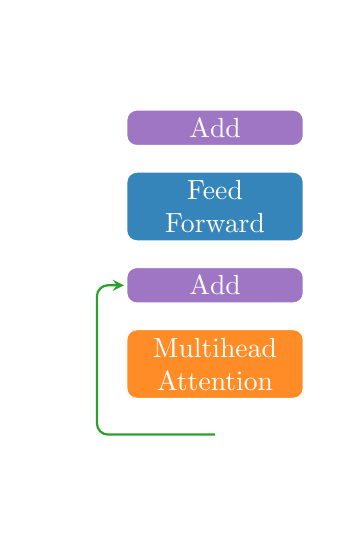
\begin{tikzpicture}[module/.style={draw, very thick, rounded corners, minimum width=15ex},
    attmodule/.style={module, fill=morange!90},
    ffnnmodule/.style={module, fill=mblue!90},
    addmodule/.style={module, fill=mpurple!90},
    arrow/.style={-stealth, thick, rounded corners},
    color = white,
]
\node (input) {Input};
\node[above of=input, attmodule, align=center, yshift=.6cm] (att) {Multihead\\Attention};
\node[above of=att, addmodule, align=center] (add1) {Add};
\node[above of=add1, ffnnmodule, align=center] (ffnn) {Feed\\Forward};
\node[above of=ffnn, addmodule, align=center] (add2) {Add};
\node[above of=add2] (output) {Output};

\draw[arrow] (input) -- (att);
\draw[arrow] (att) -- (add1); 
\draw[arrow] (add1) -- (ffnn);
\draw[arrow] (ffnn) -- (add2); 
\draw[arrow] (add2) -- (output);

\coordinate (attresidual) at ($(att.south)!0.5!(input.north)$);
\coordinate (ffnnresidual) at ($(ffnn.south)!0.5!(add1.north)$);
\coordinate[left of=add2, xshift=-.5cm] (leftofadd2);
\coordinate[left of=add1, xshift=-.5cm] (leftofadd1);
\coordinate (mhafork) at ($(att.south)!0.5!(attresidual)$);

\node[fit=(attresidual)(att)(add2)(leftofadd2),draw, ultra thick, rounded corners, label=left:$\mathrm{L\times}$] (encoder) {};
\draw[arrow, mgreen] (attresidual)-|(leftofadd1)--(add1);
\draw[arrow] (ffnnresidual)-|(leftofadd2)--(add2);
\draw[arrow] (mhafork) -|($(att.south)!0.5!(att.south west)$);
\draw[arrow] (mhafork) -|($(att.south)!0.5!(att.south east)$);
\end{tikzpicture}
\end{document}